\documentclass[12pt]{article}
\usepackage[utf8]{inputenc}
\usepackage{a4}
\usepackage[none]{hyphenat} %hyphenation
\sloppy
\usepackage{cite} 
\usepackage{parskip} %no indentation after paragraphs
\usepackage{umlaute}
\usepackage{afterpage} %for using \afterpage{\clearpage} (don't push images to the end of a chapter)
\usepackage{makeidx}
\usepackage[numbers]{natbib}
\usepackage{graphicx}
\usepackage{picins} %provides precise control over the placement of inline graphics
\usepackage{setspace}
\usepackage{titlesec}
\usepackage{dsfont} %math symbols
\usepackage{tabularx}
\usepackage{floatflt} %float text around figures and tables
\usepackage{subcaption}
\usepackage{amsthm}
\usepackage[hidelinks]{hyperref}
\usepackage{xcolor}
\hypersetup{
    colorlinks,
    linkcolor={red!50!black},
    citecolor={blue!50!black},
    urlcolor={blue!80!black}
}

% Florian Schulze, 06.06.2012
% v1.0, latest edit: 06.06.2012

\usepackage{enumitem} %resume counting from previous enumerate block
\usepackage{amsmath,amssymb}
\usepackage[format=default,font=footnotesize,labelfont=bf]{caption}
\usepackage{listings} %for listing source code
\usepackage{color}
\usepackage{algpseudocode} %for listing pseudocode
\usepackage{algorithm} %wrap algpseudocode and enrich with label etc.
\usepackage{float} % for [H] after floats

%Declare custom math operathors

\DeclareMathOperator*{\argmin}{arg\,min}
\DeclareMathOperator*{\argmax}{arg\,max}
\DeclareMathOperator{\E}{\mathbb{E}}


\titleformat{\paragraph}[hang]{\normalfont\bfseries}{\theparagraph}{.5em}{}

\makeindex
\frenchspacing
\sloppy

\pagestyle{headings}

\textwidth16cm
\textheight22cm

\topmargin0cm
\oddsidemargin0cm
\evensidemargin0cm

\newcommand{\bildklein}[3]{  
	\begin{figure}[hp]
	\begin{center}
	\includegraphics[width=0.5\textwidth]{#1}
	\end{center}
	\caption[#2]{#3}
	\end{figure}
}
  	
\newcommand{\bildgross}[3]{  
	\begin{figure}[hp]
	\begin{center}
	\includegraphics[width=0.95\textwidth]{#1}
	\end{center}
	\caption[#2]{#3}
	\end{figure}
}
  

\newcommand{\eqn}[3]{
	\begin{figure}[hp]
	\begin{equation}#1\end{equation}
	\caption[#2]{#3}
	\end{figure}
}

% This is tumlogo.tex
%
% Neues TUM-Logo in TeX
%   by G. Teege, 19.10.89
% Benutzung:
%   Am Anfang des Dokuments (TeX oder LaTeX):
%     \input tumlogo
%   Dann beliebig oft:
%     \TUM{<breite>}
%   bzw.
%     \oTUM{<breite>}
%   \TUM setzt das Logo mit der Breite <breite> und der entsprechenden Hoehe.
%   <breite> muss eine <dimen> sein. \oTUM erzeugt eine "outline"-Version
%   des Logos, d.h. weiss mit schwarzem Rand. Bei \TUM ist es ganz schwarz.
%   \oTUM entspricht damit der offiziellen Version des Logos.
%   Das Logo kann wie ein einzelnes Zeichen verwendet werden.
%   Beispiel:
%     Dies ist das TUM-Logo: \oTUM{1cm}.
%
\def\TUM#1{%
\dimen1=#1\dimen1=.1143\dimen1%
\dimen2=#1\dimen2=.419\dimen2%
\dimen3=#1\dimen3=.0857\dimen3%
\dimen4=\dimen1\advance\dimen4 by\dimen2%
\setbox0=\vbox{\hrule width\dimen3 height\dimen1 depth0pt\vskip\dimen2}%
\setbox1=\vbox{\hrule width\dimen1 height\dimen4 depth0pt}%
\setbox2=\vbox{\hrule width\dimen3 height\dimen1 depth0pt}%
\setbox3=\hbox{\copy0\copy1\copy0\copy1\box2\copy1\copy0\copy1\box0\box1}%
\leavevmode\vbox{\box3}}
%
\def\oTUM#1{%
\dimen1=#1\dimen1=.1143\dimen1%
\dimen2=#1\dimen2=.419\dimen2%
\dimen3=#1\dimen3=.0857\dimen3%
\dimen0=#1\dimen0=.018\dimen0%
\dimen4=\dimen1\advance\dimen4 by-\dimen0%
\setbox1=\vbox{\hrule width\dimen0 height\dimen4 depth0pt}%
\advance\dimen4 by\dimen2%
\setbox8=\vbox{\hrule width\dimen0 height\dimen4 depth0pt}%
\advance\dimen4 by-\dimen2\advance\dimen4 by-\dimen0%
\setbox4=\vbox{\hrule width\dimen4 height\dimen0 depth0pt}%
\advance\dimen4 by\dimen1\advance\dimen4 by\dimen3%
\setbox6=\vbox{\hrule width\dimen4 height\dimen0 depth0pt}%
\advance\dimen4 by\dimen3\advance\dimen4 by\dimen0%
\setbox9=\vbox{\hrule width\dimen4 height\dimen0 depth0pt}%
\advance\dimen4 by\dimen1%
\setbox7=\vbox{\hrule width\dimen4 height\dimen0 depth0pt}%
\dimen4=\dimen3%
\setbox5=\vbox{\hrule width\dimen4 height\dimen0 depth0pt}%
\advance\dimen4 by-\dimen0%
\setbox2=\vbox{\hrule width\dimen4 height\dimen0 depth0pt}%
\dimen4=\dimen2\advance\dimen4 by\dimen0%
\setbox3=\vbox{\hrule width\dimen0 height\dimen4 depth0pt}%
\setbox0=\vbox{\hbox{\box9\lower\dimen2\copy3\lower\dimen2\copy5%
\lower\dimen2\copy3\box7}\kern-\dimen2\nointerlineskip%
\hbox{\raise\dimen2\box1\raise\dimen2\box2\copy3\copy4\copy3%
\raise\dimen2\copy5\copy3\box6\copy3\raise\dimen2\copy5\copy3\copy4\copy3%
\raise\dimen2\box5\box3\box4\box8}}%
\leavevmode\box0}
% End of tumlogo.tex



\begin{document}

\nocite{*} %include uncited references in bibliography
\hoffset=5mm
\thispagestyle{empty}

\begin{center}
	\bigskip \bigskip \bigskip 
	\oTUM{6.0cm} \\
	\vspace*{0.8cm}
	{\huge \bf Technische Universität} \\
	\bigskip
	{\huge \bf München} \\
	\bigskip \bigskip \bigskip
	{\huge \bf Fakultät für Informatik} \\
	\bigskip \bigskip \bigskip
	{\Large \bf Master's Thesis in Informatik} \\
	\bigskip \bigskip \bigskip \bigskip \bigskip
	{\Large An Email-Centered Approach to Intelligent Task Management Using Crowdsourcing and Natural Language Processing} \\        
	\bigskip \bigskip \bigskip \bigskip
	{\Large John Doe} \\    
	\bigskip
	\begin{figure}[ht]
	\centering 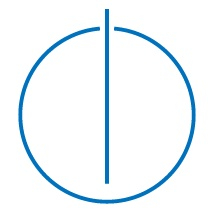
\includegraphics[width=0.2\linewidth]{figures/infologo.jpg}
	\end{figure}
	\bigskip 
\end{center}

\vfill

\newpage
\hoffset=5mm
\thispagestyle{empty}

\begin{center}
	\bigskip \bigskip \bigskip 
	\oTUM{6.0cm} \\
	\vspace*{0.8cm}
	{\huge \bf Technische Universität} \\
	\bigskip
	{\huge \bf München} \\
	\bigskip \bigskip \bigskip
	{\huge \bf Fakultät für Informatik} \\
	\bigskip \bigskip \bigskip
	{\Large \bf Master's Thesis in Informatik} \\
	\bigskip \bigskip \bigskip \bigskip \bigskip
	{\Large An Email-Centered Approach to Intelligent Task Management Using Crowdsourcing and Natural Language Processing} \\
	\bigskip \bigskip \bigskip
	{\Large Ein Email-basierter Ansatz für intelligente Aufgabenverwaltung mit Hilfe von Crowdsourcing und Natural Language Processing} \\
	\bigskip
\end{center}
\vfill

\begin{tabular}{ll}
{\Large \bf Author:} & {\Large Oleksandr Melkonyan} \\\\
{\Large \bf Supervisor:} & {\Large Prof. Dr. Johann Schlichter} \\\\
{\Large \bf Advisor:} & {\Large Dr. Wolfgang Wörndl} \\\\
{\Large \bf Submission:} & {\Large DD.MM.YYYY}
\end{tabular}

\newpage	
\thispagestyle{empty}
\hoffset=0mm
\vspace*{\fill}
\noindent I assure the single handed composition of this master's thesis only supported by declared resources.\\\\
München, DD.MM.YYYY\\\\\\\\\\\\
\noindent \textit{(Oleksandr Melkonyan)}

\newpage
\thispagestyle{empty}
\null

\newpage
\thispagestyle{empty}
\hoffset=0mm
\section*{Abstract}	
\begin{spacing}{1.2}
While providing impressive results in such domains as image and music generation, generative adversarial networks have proven to be sensitive to the choice of hyper-parameters and hard to evaluate. First problem was tackled by the authors of the Wasserstein GAN, who introduced a new loss function based on the Earth Mover distance between the generated and the real data distributions. The evaluation problem remains an open issue. Several methods have been proposed to automatically evaluate performance of GANs, including the generative adversarial metric which allows to compare two GANs and tell which one produces better results. In this work I provide an implementation of the Wasserstein GAN and compare it to a plain GAN, which uses cross-entropy loss function, using a modified version of the generative adversarial metric. Furthermore, I provide some insights about the function learned by GAN discriminator by providing different images it considers to be real, but which do not look real for a human. 
\end{spacing}
	
%\section*{Inhaltsangabe}
%\begin{spacing}{1.2}
%Deutsches Abstract.
%\end{spacing}

\newpage
\setcounter{page}{1}
\hoffset=0mm
%\bibliographystyle{wmaainf} % quotation style
\setcounter{tocdepth}{3}
\setcounter{secnumdepth}{3}
\fboxsep 0mm

\tableofcontents

\newpage
\setlength{\baselineskip}{3ex}

\begin{spacing}{1.15}
	\section{Introduction}
After their introduction in 2014 by Ian Goodfellow generative adversarial networks (GANs) have become the subject of an intensive research~\cite{gan}. Generative adversarial networks belong, as the name suggests, to the class of generative models. Such models try to learn the underlying probability distribution of the observed data. Once learned, this distribution can be used to generate new, realistic samples of data, which, depending on the training dataset, could be an image of a human face, a piano melody or a piece of poetry. Generative adversarial networks also introduced us to new problems, not common for discriminative models. The first one of these problems is the unstable training. GANs have proven to be very sensitive to the choice of hyper-parameters and the network architecture~\cite{wgan}. The newly proposed WassersteinGAN (WGAN) aims to relax this sensitivity by providing a new type of loss function, which allows to train a wider variety of networks and spend less time finding a perfect set of hyper-parameters~\cite{wgan}. Another problem inherent to GANs is that the quality of the data produced by a network is hard to evaluate automatically. This together with the fact that new GAN architectures emerge weekly makes it hard to compare all of them to choose the state-of-the-art one. In the case of discriminative models with labeled data, like image classification, evaluation of network performance is a straightforward task. One could simply run a network on a test dataset and count the number of correctly classified images. This is not possible with generative models, that produce some new, unseen data. The process of judging the quality of this data is hard to automate and sometimes it is easier to do it manually. Of coarse, the problem with manual approach is that it is not entirely objective and does not scale. Still, there is no standard framework for evaluating performance of different GAN architectures. While several different techniques have been proposed~\cite{gam, inception}, many researchers demonstrate their results by providing multiple samples generated by their GAN implementation~\cite{dcgan}. \\ 
\indent In this thesis I have implemented two deep convolutional generative adversarial networks (DCGANs) with both cross-entropy and Wasserstein loss functions respectively. Both these networks were trained on CelebA dataset to generate realistic human faces~\cite{celeba}. Then I tried to compare their performance by using a modification of the generative adversarial metric (GAM). Furthermore, I have investigated the function learned by the GAN discriminator trying to identify whether it really understands how to distinguish real data from the fake one. 
	\section{Theory background}
This section provides the required theoretical background on GANs in general and Wasserstein GAN in particular. 
\subsection{Generative adversarial networks (GANs)}
The goal of generative adversarial networks is to produce realistic data samples by learning from a given data set $D$. This can be accomplished by learning the underlying probability distribution of the data set $P_r$, the "real" probability distribution.

There are two approaches for learning $P_r$:
\begin{enumerate}
	\item To learn $P_r$ directly by defining a parametrized $P_\theta$ and finding parameters $\theta$ using the \textit{maximum likelihood estimation} (MLE)
	\item To use an input noise variable $z$ with a known probability density function $p_z(z)$ and define a parametrized mapping function $g_\theta: Z \rightarrow D$. Then, the density function of generated samples in denoted by $p_g(g_\theta(z))$. 
\end{enumerate}

While the first approach seems more straightforward, there are some flows in it. Maximizing the mean logarithm of the objective function $MLE(\theta)$ is equivalent to minimizing the \textit{Kullback-Leibler divergence}\footnote{Kullback-Leiber divergence is a measure of how one probability distribution divergence from a second one and is defined by $KL(P \lVert Q) = \int_{x} p(x) \log \frac{p(x)}{q(x)} dx$} between the two distributions $KL(P_r \lVert P_\theta)$:

\begin{align*}
	\lim_{m \to \infty} \max_{\theta} \frac{1}{m} \log MLE(\theta)
	&= \max_\theta \int_x p_r(x) \log p_\theta(x) dx \\
	&= \min_\theta - \int_x p_r(x) \log p_\theta(x) dx \\
	&= \min_\theta \int_x p_r(x) \log p_r(x) dx - \int_x p_r(x) \log p_\theta(x) dx \\
	&= \min_\theta KL(P_r \lVert P_\theta)
\end{align*}

If there is at least one data point $x \in P_r$ which has $p_\theta(x) = 0$, then the KL-divergence will immediately be infinitely large. This is a common scenario in practice, because $P_\theta$ tries to find a low dimensional manifold in the space of the observed data, and there are points lying outside of this manifold. In practice, a workaround to this problem is to add noise term $\epsilon$ to the model, to make sure that $P_\theta$ is defined everywhere. Then, the estimated probability distribution will be defined by 
\begin{equation*}
p_{estimated}(x) = \frac{p_\theta(x) + \lambda \cdot \epsilon(x)}{\int_x p_\theta(x) + \lambda \cdot \epsilon(x) dx}, 
\end{equation*}
where $\lambda$ is the amount of noise we want to add to the model. This, however, is not an ideal solution because it degrades the sample quality. \\
  
\indent Generative adversarial networks implement the latter approach with a mapping function $g_\theta$ being encoded using a neural network, called \textit{generator} $G$. Instead of the MLE generative adversarial networks use \textit{adversarial training} to find parameters for the generator. To measure the quality of the generator $G$ another network is used, the \textit{discriminator}, which takes an input sample and outputs the probability that the sample comes from the real data set. The architecture of a GAN is shown in Figure~\ref{fig:gan}.\\

\begin{figure}[h]
	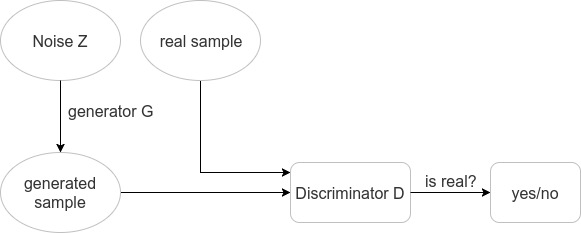
\includegraphics[width=\textwidth]{figures/gan}
	\caption{A visualization of how different parts of a GAN are connected with each other. A generator network $G$ produces samples from a noise variable $Z$. A discriminator network $D$ takes both real and generated samples and tries to distinguish between them.}
	\label{fig:gan}
\end{figure}

\indent In order to train a GAN model one has to define two loss functions. One that quantifies how well a discriminator $D$ can distinguish between a real probability distribution $p_r(x)$ and its approximation computed by a generator $G$, $p_g(G(z))$. Second loss function evaluates how well the generator can approximate the real distribution. For a standard GAN these loss functions are defined as: 
\begin{equation} \label{eq:gan_loss}
\argmin_G \argmax_D L(G,D) = \E_{x \sim p_r(x)} [\log(D(x)] + \E_{z \sim p_z(z)}[\log(1-D(G(z))]
\end{equation}
Let us analyze equation~\ref{eq:gan_loss} from the viewpoint of a discriminator. The maximum value of $L(G,D)$ is achieved when both $\E_{x \sim p_r(x)} [\log D(x)]$ and $\E_{z \sim p_z(z)}[\log(1-D(G(z)))]$ are equal to zero. For this to hold, the values inside of the  logarithms should be equal to one. This means that the discriminator should output one for real samples and zero for generated ones. When optimizing with respect to the generator the first term of equation~\ref{eq:gan_loss} is constant. And the term $\E_{z \sim p_z(z)}[\log(1-D(G(z))]$ is equal to zero when the discriminator thinks that the samples generated by the generator are real. There is no closed form solution for~\ref{eq:gan_loss} and the most common method of optimization is by applying a gradient descent to the generator and to discriminator alternately.\\  

\indent A natural question that arises after looking at the adversarial training procedure is how it relates to measuring distance between the real distribution $P_r$ and the generated one $P_G$. 

First observation is that with a generator $G$ fixed, optimal discriminator $D$ is equal to
\begin{equation}
	D^*(x) = \frac{p_r(x)}{p_r(x) + p_g(x)}
\end{equation}
\begin{proof}
	\begin{align*}
		L(G, D) &= \int_x p_r(x)\log(D(x))dx + \int_z p_z(z)\log(1 - D(G(z))) dz \\
		&= \int_x p_r(x)\log(D(x))dx + \int_x p_g(x)\log(1 - D(x)) dx
	\end{align*}
The minimal value of a function $a\log(y) + b\log(1-y)$ is achieved at the point $y = \frac{a}{a+b}$ for all $(a,b) \in \mathbb{R}^2 \setminus (0,0)$. This can be shown by finding a null point of the corresponding derivative $\frac{a}{y} - \frac{b}{1-y}$.
\end{proof}

Now with an optimal discriminator $D^*$ we can rewrite $L(G,D)$ as following
\begin{align*}
	L(G, D) &= \E_{x \sim p_r(x)} [\log(D^*(x)] + \E_{z \sim p_z(z)}[\log(1-D^*(G(z))] \\
	&= \E_{x \sim p_r(x)} [\log(D^*(x)] + \E_{x \sim p_g}[\log(1-D^*(x)] \\
	&= \E_{x \sim p_r(x)} \bigg[\log \frac{p_r(x)}{p_r(x) + p_g(x)}\bigg] + \E_{x \sim p_g}\bigg[\log \frac{p_g(x)}{p_r(x) + p_g(x)}\bigg] \\
	&= -\log 4 + \E_{x \sim p_r(x)} \bigg[\log \frac{p_r(x)}{\frac{p_r(x) + p_g(x)}{2}}\bigg] + \E_{x \sim p_g}\bigg[\log \frac{p_g(x)}{\frac{p_r(x) + p_g(x)}{2}}\bigg] \\
	&= -\log 4 + KL\bigg(P_r \lVert \frac{P_r + P_g}{2}\bigg) +  KL\bigg(P_g \lVert \frac{P_r + P_g}{2}\bigg) \\
	&= -\log 4 + 2 \cdot JSD(P_r \lVert P_g),
\end{align*}
where $JSD(P_r \lVert P_g)$ is the \textit{Jensen-Shannon divergence}  \footnote{Jensen-Shannon divergence is a distance measure between two probability distributions and is defined by $JS(P\lVert Q) = \frac{1}{2} KL(P \lVert \frac{P+Q}{2}) +\frac{1}{2} KL(Q \lVert \frac{P+Q}{2})$, where KL denotes the Kullback-Leibler divergence.} between two distributions. Since the JS divergence is defined everywhere, this approach does not suffer from the problems described for the MLE.

We have shown that assuming that a discriminator is always trained to optimality, objective function defined in equation~\ref{eq:gan_loss} can be interpreted as a Jensen-Shannon divergence between the real distribution $P_r$ and the one approximated by a generator $P_g$.  

The training process of a GAN consists of the following steps:
\begin{enumerate}
	\item With a fixed generator train a discriminator to optimality.
	\item With an optimal discriminator, train the generator. 
	\item Repeat previous steps. Knowing when to stop the training process is not trivial and will be discussed in the following sections.
\end{enumerate}
Since we can not compute $\E_{x \sim p_r(x)} [\log(D(x)]$ we approximate in by 
\begin{equation}
	\frac{1}{m} \sum_{i=1}^{m} D(x_i),
\end{equation}
where $x_i$ is a random subset of training samples, $m$ is usually small compared to the number of training samples available. This technique is called \textit{stochastic gradient descent}. The same is done to compute $\E_{z \sim p_z(z)}[\log(1-D(G(z))]$.
 
\subsection{Wasserstein GANs (WGANs)}
Wasserstein GANs were introduced in January 2017~\citep{wgan}. The authors argue that the Jensen-Shannon divergence, used in original GANs to calculate the distance between generated and original probability distributions, has some problems and proposed a new objective function based on the \textit{Earth-Mover} (EM)  distance. This distance should improve stability of the training process and provide a distance measure that corresponds to the perceived sample quality. 
	The Earth-Mover distance between two distributions is defined by
\begin{equation}
	W(P_g, P_r) =  \inf_{\gamma \in \prod (P_r, P_g)}  \E_{(x,y) \sim \gamma} [ \lVert x - y \lVert_2 ],
\end{equation}
where $\prod (P_r, P_g)$ is a set of all joint distributions $\gamma(x,y)$ whose marginal distributions are $P_r$ and $P_g$ respectively. To understand the idea behind the EM distance we can imagine that probability distributions assign a mass to each point $x$ and we want to turn distribution $P_r$ into $P_g$ by moving this mass around. Furthermore, moving a mass $m$ by a distance $d$ would cost us $m \cdot d$ effort. In this imaginary scenario the EM distance will give us the minimal effort we would have to spend. Why is this true? 
\begin{itemize}
	\item We can think of each $\gamma(x, y)$ as the amount of mass transported between points $x$ and $y$, then in our scenario $\gamma$ will represent a "transport plan" for transitioning from $P_r$ to $P_g$.
	\item For $\gamma$ to be a valid strategy it has to satisfy several conditions:
		\subitem Amount of mass leaving point $x$ is calculated by $\int_y \gamma(x, y) dy$ and should be equal to $p_r(x)$, the amount of mass originally located at $x$
		\subitem In the same way, the amount of mass entering $y$ is calculated by $\int_x \gamma(x, y) dx$ and should be equal to $p_g(y)$, the amount of mass located at $y$ at the end.
	\item These conditions mean that marginal distributions of $\gamma(x, y)$ should equal to $P_r$ and $P_g$ respectively. 
	\item The amount of effort required to execute the transporting plan $\gamma$ is 
	\begin{equation}
	\int_x \int_y \gamma(x,y) \lVert x - y \lVert_2 dx dy = \E_{(x,y) ~\sim \gamma} [ \lVert x - y \lVert_2 ]
	\end{equation}
	\item Infinum over this effort gives the EM distance. 
\end{itemize}

One property that is expected from an objective function is that it is continuous and differentiable in its whole domain. And this is exactly where EM distance outperforms the Jensen-Shannon divergence, which is illustrated in the following example, taken from the original paper. 

Consider a uniform random variable $Z \in [0, 1]$. Let $P_r$ be the distribution of a random variable $(0, Z) \in \mathbb{R}^2$. Let $g_\theta: \mathbb{R} \rightarrow \mathbb{R}^2$, $g_\theta(z) = (\theta, z)$ be a mapping function with a single parameter $\theta$. Now we can compute the Jensen-Shannon divergence and the EM distance between $P_r$ and $P_g$. 
To compute the Jensen-Shannon divergence we first need to compute $KL(P_r \lVert M)$ where $M = \frac{1}{2}P_r + \frac{1}{2}P_g$:
\begin{equation}
	KL(P_r \lVert M) = \int_{x,y} p_r(x,y) \log \frac{p_r(x,y)}{m(x,y)} dxdy = \log2,
\end{equation}
because $m(x,y) = \frac{1}{2} p_r(x,y)$ everywhere except for points with $x=0$ or $x=\theta$. The same is true for $KL(P_g \lVert M)$ and therefore:
\begin{align*}
 JSD(P_r \lVert P_g) &= \frac{1}{2}KL(P_r \lVert M) + \frac{1}{2}KL(P_g\lVert M) \\ 
 	&= \begin{cases}
 		\log2, & \text{if } \theta \neq 0 \\
 		0, & \text{if } \theta = 0
 	\end{cases}.
\end{align*}  
On the other hand, if we recall the example explaining the intuition behind the ME distance, we can see that to transport all the mass from $P_r$ to $P_\theta$ we need to transport each mass point by distance $\theta$, therefore
\begin{equation}
	M(P_r, P_g) = \int_{(0,z)} |\theta| \cdot p_r(0,z)dz = |\theta|
\end{equation}

Already from this example we can see that there are cases where the EM distance is continuous whilst JS divergence not. Authors have shown that if a mapping function $g_\theta(x)$ is itself continuous, so that is the EM distance $M(P_r, P_g)$. Moreover, if $g_\theta(x)$ fulfills certain criteria, EM distance will be differentiable almost in the whole domain. At the same time, both statements are false for the JS divergence~\citep{wgan}. The criteria for the function $g_\theta(x)$ to be fulfilled are:
\begin{enumerate}
	\item The function $g_\theta$ is \textit{locally Lipschitz continuous}. \\
	A real-valued function $g_\theta$ is called Lipschitz continuous if there exists a constant $K$, called a \textit{Lipschitz constant}, such that for all $x_1$ and $x_2$:
	\begin{equation}
		\lVert g_\theta(x_1) - g_\theta(x_2) \lVert_2 \leq K\lVert x_1 - x_2 \lVert_2
	\end{equation}  
	Local Lipschitz continuity means that for each point $x$ there exists a neighborhood $U$ where $g_\theta$ is Lipschitz continuous. \\
	In other words, Lipschitz continuity restricts how fast a function can change, because the inclination angle of the line connecting \textbf{each} two points of the function(and thus the value of derivatives) is restricted by a constant $K$. 
	\item The function $g_\theta$ satisfies \textit{regularity assumption 1}. \\
	Let $K(\theta, z)$ denote the local Lipschitz constant at point $(\theta, z)$ of a locally Lipschitz continuous function $g_\theta(z)$. Then, $g_\theta$ satisfies the regularity assumption 1 if the expected value of $K(\theta, z)$ is upper-bounded:
	\begin{equation}
		\E_z[K(\theta, z)] < +\infty
	\end{equation}
\end{enumerate} 
While these assumptions are tedious to prove manually for each mapping function $g_\theta$, authors have shown that all feed-forward neural networks with pointwise or rectified nonlinearities satisfy both these requirements and therefore when using such networks to encode a  generator of a GAN, the EM distance will be continuous and differentiable almost everywhere.  

To utilize the properties of the EM distance we should be able to compute it efficiently. Unfortunately, computing it exactly is not feasible, therefore we have to approximate. 
Firstly, we can use the Kantorovich-Rubinstein duality to rewrite $W(P_r, P_\theta)$ as following
\begin{equation}
	W(P_r, P_\theta) = \sup_{\lVert f \lVert_L \leq 1} \E_{x \sim P_r}[f(x)] - E_{x \sim P_\theta} [f(x)],	
\end{equation}
where ${\lVert f \lVert_L \leq 1}$ denotes the set of all functions that are Lipschitz continuous with Lipschitz constant equal $1$, or also called \textit{1-Lipschitz} functions. If we replace this set with ${\lVert f \lVert_L \leq K}$ we will receive the upper bound for $K \cdot W(P_r, P_\theta)$ instead, which is still intractable to compute but easier to approximate. As already discussed, a discriminator $D$  encoded using a neural network with parameters $w$ is a $K$-Lipschitz function. Therefore
\begin{align*}
\max_w \E_{x \sim P_r}[D(x)] - E_{x \sim P_\theta} [D(x)] &\leq \sup_{\lVert D \lVert_L \leq K} \E_{x \sim P_r}[D(x)] - E_{x \sim P_\theta} [D(x)] \\
 &= K \cdot W(P_r, P_\theta)
\end{align*}
Note, that supremum may not be achieved, if there is a $K$-Lipschitz function that can not be encoded with parameters $\theta$ or if the supremum is achieved for some $k$-Lipschitz function with $k < K$.

One thing that is remained to do is to ensure that $K$ remains constant during the training process. One obvious way to do that is to restrict the space $S$ of possible functions encoded by $D$, then the set of possible Lipschitz constants will be upper-bounded. We enforce discriminators to lie in $S$ by defining an upper and a lower bound for all weights of a discriminant, which will remain unchanged throughout the training process. This process is called \textit{weight clipping}.
 
To train the discriminator we have to compute the gradients of $W(P_r, P_\theta)$ with respect to $w$:
\begin{align*}
	\nabla_w W(P_r, P_\theta) &= \nabla_w(\E_{x \sim P_r}[D_w(x)] - E_{z \sim Z} [D_w(G_\theta(z))]) \\
&= \E_{x \sim P_r}[\nabla_w(D_w(x))] - \E_{z \sim Z} [\nabla_w(D_w(G_\theta(z)))]
\end{align*} 
In the same way, updates for Generator $G$ are obtained by computing the gradients with respect to $\theta$ 
\begin{align*}
\nabla_\theta W(P_r, P_\theta) &= \nabla_\theta(\E_{x \sim P_r}[D_w(x)] - E_{z \sim Z} [D_w(G_\theta(z))]) \\
&= - \E_{z \sim Z} [\nabla_\theta D_w(G_\theta(z))]
\end{align*}

The training process therefore consists of the following steps:
\begin{enumerate}
	\item For a fixed generator train the discriminator to the convergence in order to obtain an approximation of $W(P_r, P_\theta)$:
	\begin{enumerate}
		\item Update discriminator's weights using computed gradient.
		\item Enforce the discriminator to remain $K$-Lipschitz by clipping its to values $[-c, c]$, where $c$ remains constant during the training process.
	\end{enumerate}	
	\item With an optimal discriminator update the generator by computing the gradient $- \E_{z \sim Z} [\nabla_\theta D(G(z))]$	
\end{enumerate}

\begin{figure}[h]
  \begin{subfigure}[b]{0.5\textwidth}
    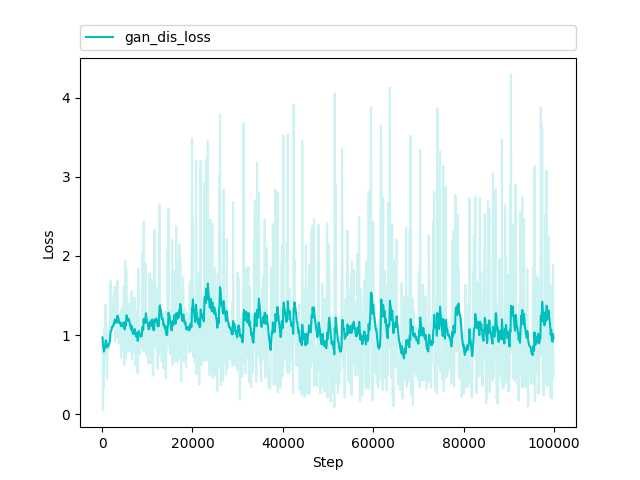
\includegraphics[width=\textwidth]{figures/gan_dis_loss}
    \caption{GAN discriminator loss}
    \label{fig:gan_dis_loss}
  \end{subfigure}
  \hfill
  \begin{subfigure}[b]{0.5\textwidth}
    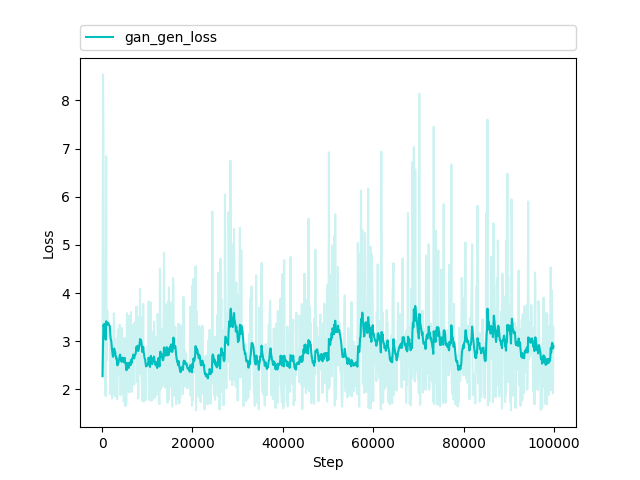
\includegraphics[width=\textwidth]{figures/gan_gen_loss}
    \caption{GAN generator loss}
    \label{fig:gan_gen_loss}
  \end{subfigure}
  \begin{subfigure}[b]{0.5\textwidth}
    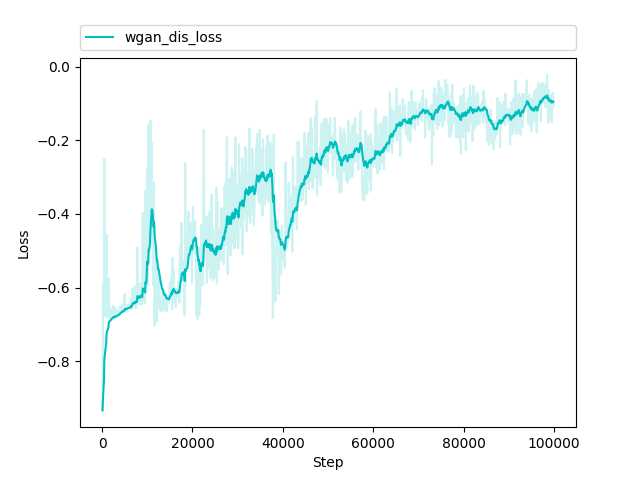
\includegraphics[width=\textwidth]{figures/wgan_dis_loss}
    \caption{Wasserstein GAN discriminator loss}
    \label{fig:wgan_dis_loss}
  \end{subfigure}
  \hfill
  \begin{subfigure}[b]{0.5\textwidth}
    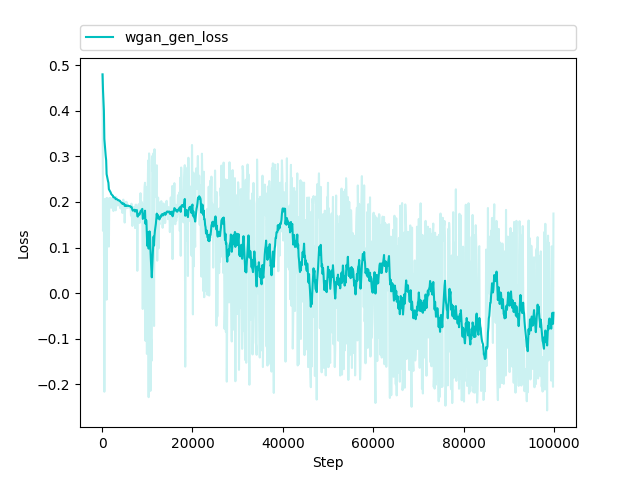
\includegraphics[width=\textwidth]{figures/wgan_gen_loss}
    \caption{Wasserstein GAN generator loss}
    \label{fig:wgan_gen_loss}
  \end{subfigure}
  
  \caption{Figures illustrating that WGAN has a correlation between the number of training steps and the values of its objective functions. On the other hand the objective functions of a GAN remain in the same interval although the quality of the samples increases.}
  \label{fig:losses}
\end{figure}
\begin{figure}[h]
  \begin{subfigure}[b]{\textwidth}
    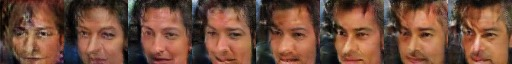
\includegraphics[width=\textwidth]{figures/gan_progress}
    \caption{Evolution of GAN generated samples quality}
    \label{fig:gan_evolution}
  \end{subfigure}
  \begin{subfigure}[b]{\textwidth}
    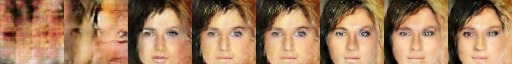
\includegraphics[width=\textwidth]{figures/wgan_progress}
    \caption{Evolution of Wasserstein GAN generated samples quality}
    \label{fig:gan_evolution}
  \end{subfigure}
  \caption{Samples generated after different number of training steps. Each sample is generated from the same noise variable.}
  \label{fig:samples_evolution}
\end{figure}

Apart from the fact that the Wasserstein GAN allows more stable training, its loss function corresponds to the image quality. This is illustrated in Figures~\ref{fig:losses} and~\ref{fig:samples_evolution}.



\subsection{Deep Convolutional GANs (DCGANs)}
So far we discussed GANs without paying attention to the architecture of underlying generator and discriminator. On the one hand, this is a powerful feature of the framework, because it allows a higher level of abstraction. It is possible to encode a generator and a discriminator using a deep convolutional neural network, an auto-encoder or every other network type. However, this choice inevitably affects the performance of the resulting GAN and therefore has to be thoroughly evaluated. In my thesis I have used deep convolutional GANs (DCGANs) because they are well suited for image generation tasks~\cite{dcgan}. In DCGANs both a generator and a discriminator are encoded convolutional neural networks (CNNs) and this section provides an overview of this network type. 

First introduced in their current form in 1996 by Yann LeCunn~\cite{lecun}, CNNs became really popular in 2012, when a CNN called AlexNet won an image recognition competition significantly improving all previous results~\cite{alexnet}. 


\begin{figure}[h]
  \begin{subfigure}[b]{0.24\textwidth}
    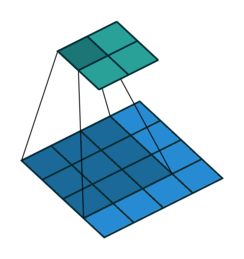
\includegraphics[width=\textwidth]{figures/no_padding_no_strides_00}
  \end{subfigure}
  \begin{subfigure}[b]{0.24\textwidth}
    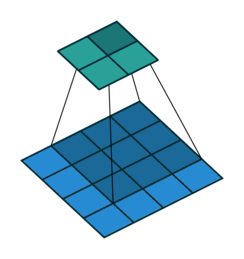
\includegraphics[width=\textwidth]{figures/no_padding_no_strides_01}
  \end{subfigure}
  \begin{subfigure}[b]{0.24\textwidth}
    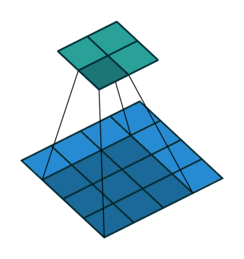
\includegraphics[width=\textwidth]{figures/no_padding_no_strides_02}
  \end{subfigure}
  \begin{subfigure}[b]{0.24\textwidth}
    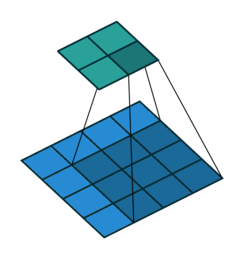
\includegraphics[width=\textwidth]{figures/no_padding_no_strides_03}
  \end{subfigure}  
  \caption{An example of a convolution filter. The lower matrix is an input layer, the upper one represents the output layer. The patches being convoluted are highlighted with a darker color.}
  \label{fig:conv_no_padding_no_strides}
\end{figure}

The core idea of CNNs is to learn hierarchies of location independent features present in an image. Features in the first layer of a CNN are just geometric primitives like edges, but last layers represent complex context dependent features like eyes or noses. Layers of a CNN are built of multiple \textit{convolution filters} that are applied to each patch of the input, as shown\footnote{All visualizations of convolution filters where generated using the code provided by the author of the paper~\cite{conv_tutorial}. The code is available on GitHub: \url{https://github.com/vdumoulin/conv_arithmetic}.} in Figure~\ref{fig:conv_no_padding_no_strides}. A convolution filter $F \in \mathbb{R}^{K \times K}$ is a matrix of weights. When applying $F$ to a patch $P$ of the input we simply compute the sum of the element-wise product between $F$ and $P$:

\begin{equation}
	F * P  = \sum_{i=1}^K \sum_{j=1}^K f_{ij} \cdot p_{ij}.
\end{equation}

\begin{figure}[h!]
  \begin{subfigure}[b]{0.32\textwidth}
    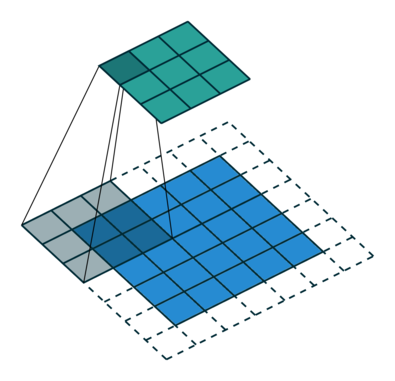
\includegraphics[width=\textwidth]{figures/padding_strides_00}
  \end{subfigure}
  \begin{subfigure}[b]{0.32\textwidth}
    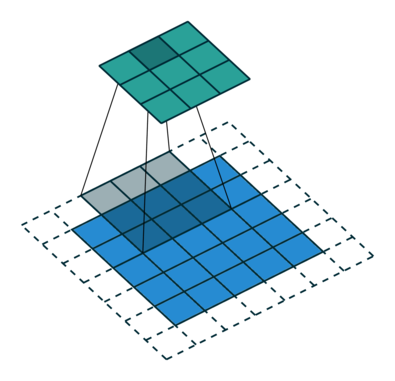
\includegraphics[width=\textwidth]{figures/padding_strides_01}
  \end{subfigure}
  \begin{subfigure}[b]{0.32\textwidth}
    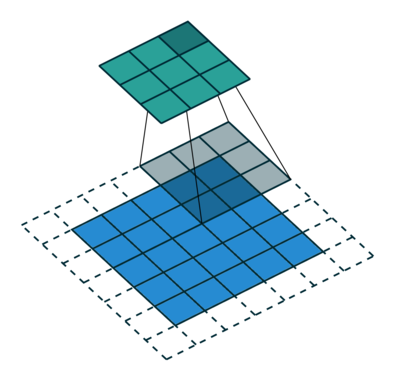
\includegraphics[width=\textwidth]{figures/padding_strides_02}
  \end{subfigure}
%  \begin{subfigure}[b]{0.32\textwidth}
%    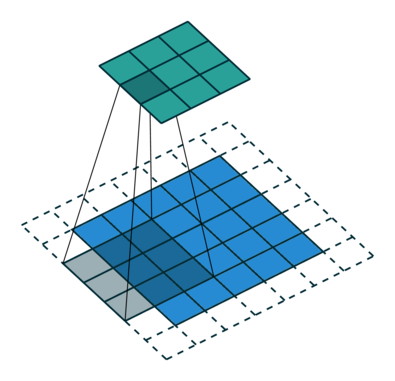
\includegraphics[width=\textwidth]{figures/padding_strides_03}
%  \end{subfigure}  
%  \begin{subfigure}[b]{0.32\textwidth}
%    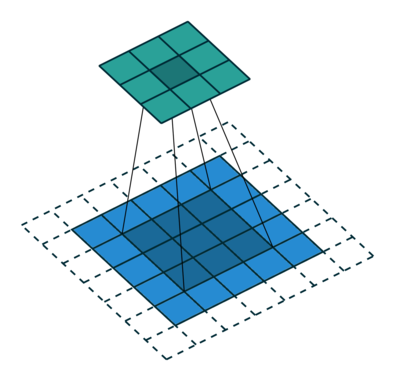
\includegraphics[width=\textwidth]{figures/padding_strides_04}
%  \end{subfigure}
%  \begin{subfigure}[b]{0.32\textwidth}
%    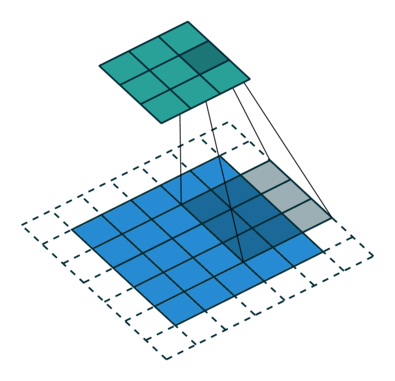
\includegraphics[width=\textwidth]{figures/padding_strides_05}
%  \end{subfigure}
%  \begin{subfigure}[b]{0.32\textwidth}
%    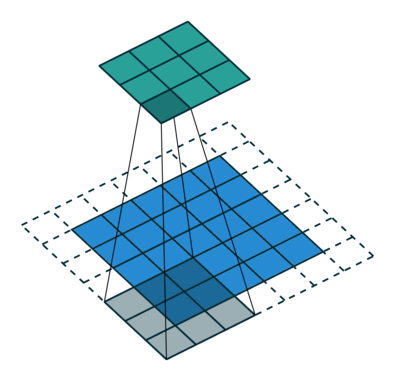
\includegraphics[width=\textwidth]{figures/padding_strides_06}
%  \end{subfigure}
%  \begin{subfigure}[b]{0.32\textwidth}
%    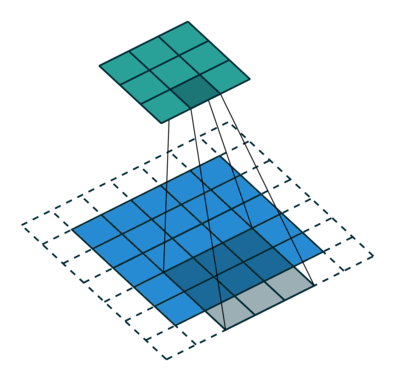
\includegraphics[width=\textwidth]{figures/padding_strides_07}
%  \end{subfigure}  
%  \begin{subfigure}[b]{0.32\textwidth}
%    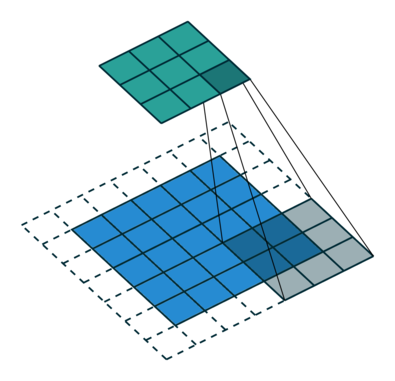
\includegraphics[width=\textwidth]{figures/padding_strides_08}
%  \end{subfigure}  
  \caption{An example of a convolution filter with padding $p=(1,1)$ and strides $s = (2,2)$. The transparent cells of the lower matrix represent padded zero elements.}
  \label{fig:conv_padding_strides}
\end{figure}

Since the same filter $F$ is applied to each patch of the input, it learns a location independent feature present there. Sometimes the input matrix is \textit{padded} with $p$ zeros to increase the number of patches. The distance between the centers of two adjacent patches is called \textit{stride} $s$, as illustrated in Figure~\ref{fig:conv_padding_strides}. Strides and padding allow to manipulate the size of the output:

\begin{equation}
	o = \Bigl\lfloor \frac{i + 2p - k}{s} \Bigr\rfloor + 1,
\end{equation}
where $i$ is the size of the input, $o$ size of the output, $k$ size of the convolution filter, $p$ and $s$ sizes of padding and strides respectively. After a convolution filter some non linear function is applied to the output. In my experiments I have used the leaky rectified linear units(leaky ReLUs): 

\begin{equation}
	f(x) = \begin{cases}
			x & \text{if }x > 0\\
			a \cdot x &\text{otherwise}
			\end{cases}	
\end{equation}

In the DCGAN generator another convolution type is used. It is called \textit{transposed convolution}. The convolution operation can be rewritten as a product of the input and a sparse matrix $C$~\cite{conv_tutorial}. Then, we can transpose $C$ to swap the input and the output. The resulting product of the input and $C^T$ can be again replaced by sliding the convolutional matrix $F$ over the input. An example of a transposed convolution is shown in Figure~\ref{fig:conv_padding_strides_transposed}. Transposed convolutions allow to increase the input dimensions while keeping the same connectivity pattern as in the convolution filter. 

\begin{figure}
	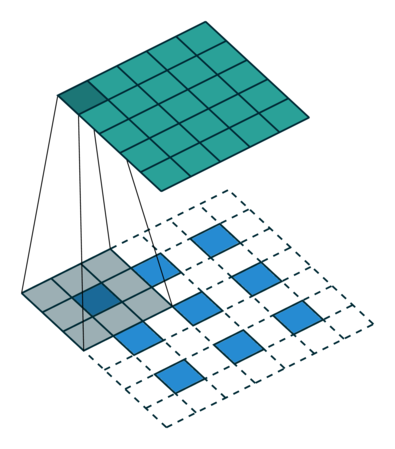
\includegraphics[width=0.18\textwidth]{figures/padding_strides_transposed_00}
	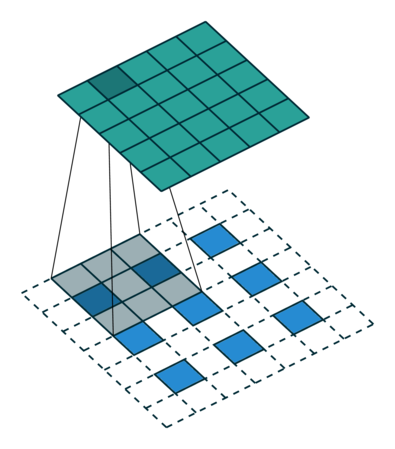
\includegraphics[width=0.18\textwidth]{figures/padding_strides_transposed_01}
	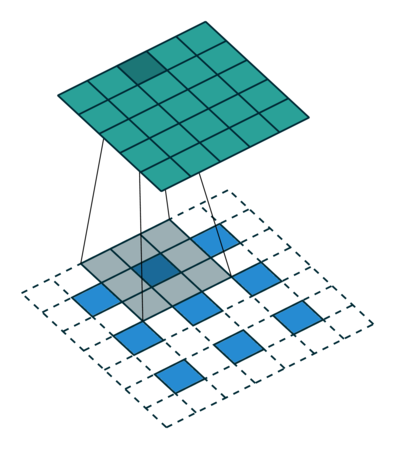
\includegraphics[width=0.18\textwidth]{figures/padding_strides_transposed_02}
	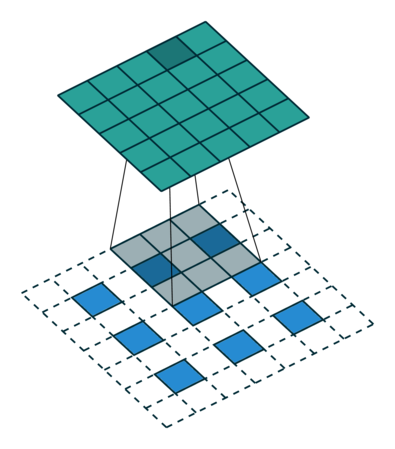
\includegraphics[width=0.18\textwidth]{figures/padding_strides_transposed_03}
	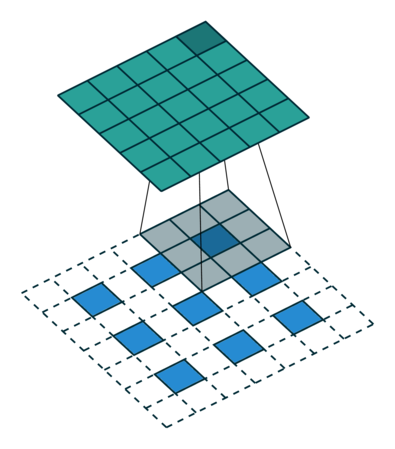
\includegraphics[width=0.18\textwidth]{figures/padding_strides_transposed_04}
	\caption{ The transpose of convolving a kernel $k=(3,3)$ over an input $i=(5,5)$ padded with $p=(1,1)$ border of zeros using strides $s=(2,2)$. It is equivalent to convolving a kernel $\tilde{k} = (3,3)$ over an input $\tilde{i} = (3,3)$ (with 1 zero inserted between inputs) padded with $p=(1,1)$, using unit strides.}
	\label{fig:conv_padding_strides_transposed}
\end{figure}

\subsection{Batch normalization}
An important technique used in the DCGAN is the \textit{batch normalization}~\cite{batch_norm}. The input of a hidden\footnote{All layers of a neural network except the first and the last ones are called hidden layers} layer is in turn the output of all previous layers. Therefore, the distribution of this input will change each time we update parameters of the previous layers, a phenomenon known as \textit{internal covariate shift}. As a consequence, parameters of the hidden layer have to be constantly adapted for a new data distribution. This can slow down the training process and make the network sensitive to the initial values of the parameters. Batch normalization modifies the input mini-batch of each layer to have zero mean and unit variance: 
\begin{align*}
	\mu &= \frac{1}{m} \sum_{i=1}^{m}x_i \\
	\sigma^2 &= \frac{1}{m} \sum_{i=1}^{m}(x_i - \mu)^2 \\
	\hat{x}_i &= \frac{x_i - \mu}{\sqrt{\sigma+\epsilon}} \\
	BN_{\gamma, \beta}(x_i) &= \gamma \hat{x}_i + \beta,
\end{align*}
where $m$ is the number of samples in the mini-batch, $\epsilon$ is a constant to improve the numeric stability, $\gamma$ and $\beta$ are two more parameters to optimize during the training process. As shown in Figure~\ref{fig:gan_arc} batch normalization is applied to the inputs of all hidden layers of the GANs used in this paper.

	\section{Evaluating GAN performance}
Evaluating performance of a discriminative model is a rather straightforward issue. One would reserve a portion of data available for a test data set and after training run the model on this data set and count the number of samples correctly classified. With generative models things get more complicated. Judging the quality of generated samples, whether these are images, text or something else, can be challenging and often subjective. However, this has to be done in order to compare different GANs regularly proposed by researches and therefore some creative ideas were proposed to tackle this problem. Some of the methods can be applied only in a particular domain, like generating images displaying multiple objects, while others can be applied to an arbitrary GAN. 
\subsection{Manual evaluation}
The best way to judge the quality of generated contend is still by using real people. For example, Ian Goodfellow \textit{et al.} have created a simple website\footnote{The website can be accessed under  \url{http://infinite-chamber-35121.herokuapp.com/cifar-minibatch/}}, showing user a number of pictures, some of which are generated and some are real. The user is then asked to choose the pictures which he or she thinks were generated by the network. Moreover, the quality of an image is also indicated by the time spent to decide whether is it real or not. Therefore, Emily Denton \textit{et al.} did several test varying the amount of time user was able to see an image before it disappeared~\cite{laplacian_gan}. If the number of positive responses declines with the increase of the amount of time available to judge an image, it is a signal of the poor image quality.
\subsection{Annealed importance sampling (AIS)}
\subsection{Inception score}

\subsection{Generative adversarial metric(GAM)} \label{sec:gam}
Generative adversarial metric (GAM) is an another way of comparing the performance of two GANs. This metric does quantify the quality of a single GAN but rather can give a hint on which of two compared networks performs better. This is done by swapping the GANs' discriminators, as shown in figure 
\begin{figure}[h]
	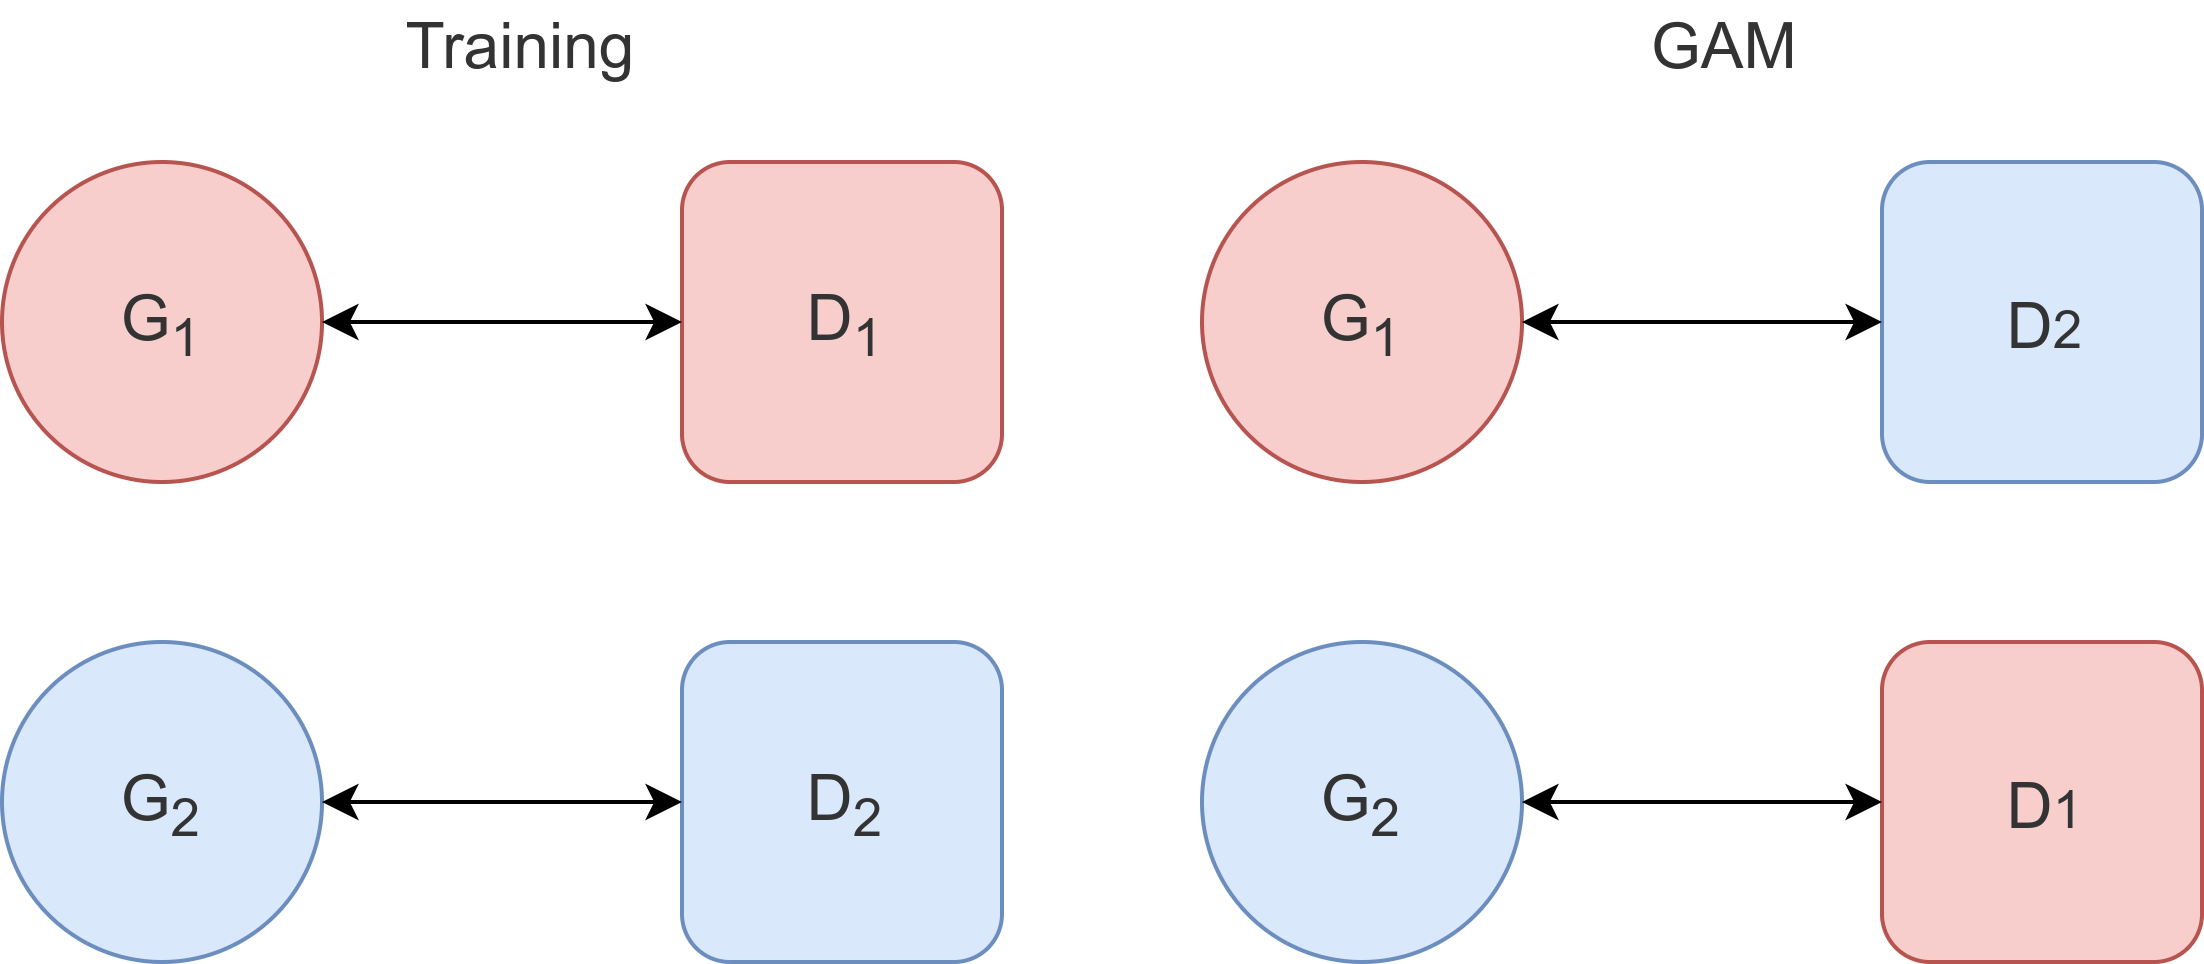
\includegraphics[width=\textwidth]{figures/gam}
	\caption{Visualization the GAM idea. First GAN consists of a generator $G_1$ and a discriminator $D_1$, the second one of $G_2$ and $D_2$ respectively. When the GAM is computed, GANs swap their discriminators, so that $D_1$ judges whether images data produced by $G_2$ look realistic or not, while $D_2$ does the same for $G_1$.}
	\label{fig:gam}
\end{figure}
 
After exchanging discriminators two quantities are computed:
\begin{align} \label{eq:gam_real}
	r_{real} &= \frac{\epsilon(D_1(x_{real}))}{\epsilon(D_2(x_{real}))} \\ 
	r_{generated} &= \frac{\epsilon(D_1(G_2(z)))}{\epsilon(D_2(G_1(z)))}, \label{eq:gam_gen} 
 \end{align}
where $\epsilon(\cdot)$ denotes the misclassification ratio which is be computed by 
\begin{equation*}
	\frac{\text{correctly classified samples}}{\text{total number of samples}}.
\end{equation*} 
Then, depending on the values of the two indicators, we can conclude which GAN performs better:
\begin{equation}
\text{winner} = \begin{cases}
	GAN_1, & \text{if } r_{generator} < 1 \text{ and } r_{real} \approx 1 \\
	GAN_2, & \text{if } r_{generator} > 1 \text{ and } r_{real} \approx 1 \\
	\text{tie}, & \text{if } r_{generator} \approx 1 \text{ and } r_{real} \approx 1  \\
	\text{undefined}, & \text{if } r_{real} \neq 1	
	\end{cases}
\end{equation}
Note that because we actually want to compare the generators, such a comparison is possible only if both discriminators perform equally well, which is indicated by the condition $r_{real} \approx 1$.  

	\section{Comparing a plain GAN and a Wasserstein GAN}

\subsection{Networks architecture}
	The discriminator and the generator in both the GAN and the WGAN are implemented using convolutional neural networks. The architecture is visualized in Figure~\ref{fig:gan_arc}. As we can see, the generator networks are identical while the architecture of the discriminators has some minor differences. For examples, the size of the convolutional filter is smaller in the WGAN discriminator. Also, the WGAN discriminator's output is not a probability of an image being real anymore but rather a $2 \times 2 \times 1 $ tensor which is solely used to compute the loss functions of the WGAN networks. As already discussed in Section~\ref{sec:batch_norm}, almost all layers of the networks have a batch normalization. Implementation of these models can be found on Github~\url{https://github.com/melkonyan/BA_WassersteinGAN}. 
\begin{figure}[h]
	\includegraphics[width=\textwidth]{figures/architecture}
	\caption{Architectures of the GAN and the WGAN used in this paper.}
	\label{fig:gan_arc}
\end{figure}
\subsection{Proposed evaluation method}
Unfortunately, the generative adversarial metric discussed in Section~\ref{sec:gam} can not be applied to compare a plain GAN with a WGAN. This is due to the fact that the output of a WGAN discriminator can not be interpreted as a probability that a sample is real. Therefore, we can not compute the $\epsilon(D_{WGAN}(x_{real}))$ and $\epsilon(D_{WGAN}(G_{GAN}(z)))$ terms of Equations~\ref{eq:gam_real} and \ref{eq:gam_gen} respectively. I have tried to use an approach inspired by the GAM but instead of computing the error rates $\epsilon(\cdot)$ on a test dataset I have plotted discriminators' losses during the training process. Here is the summarized procedure: 
\begin{enumerate}
	\item Do several training steps of both the GAN and the WGAN.
	\item Log the WGAN discriminator's performance 
		\begin{enumerate}
			\item Compute the WGAN discriminator's loss using images generated by the GAN generator.
			\item Compute the WGAN discriminator's loss using its own generator
		\end{enumerate}	
	\item Log the GAN discriminator's performance
		\begin{enumerate}
			\item Compute the GAN discriminator's loss using images generated by the WGAN generator.
			\item Compute the GAN discriminator's loss using its own generator
		\end{enumerate}
	\item Go to Step 1.
\end{enumerate}
Before taking a look at the results let us discuss possible outcomes of the procedure described above, which are visualized in Figures~\ref{fig:cd_wgan_wins},~\ref{fig:cd_equal},~\ref{fig:cd_gen_overfit},~\ref{fig:cd_dis_overfit}. 
In the normal case one of the two following scenarios will happen:
\begin{enumerate}
	\item The desired scenario, in which one of the generators produces images that are harder to distinguish for both discriminators. In this case we can assume that the generator can produce images of a better quality. An example of the corresponding loss curves is shown in Figure~\ref{fig:cd_wgan_wins}.	
	\item If both generators perform equally well, all the loss curves will be approximately identical, as shown in Figure~\ref{fig:cd_equal}.
\end{enumerate}

	\begin{figure}[h!] 
		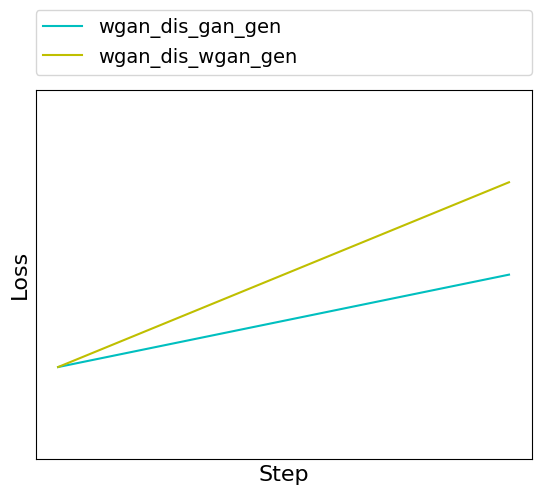
\includegraphics[width=0.5\textwidth]{figures/ex/wgan_wins_wgan_dis}
		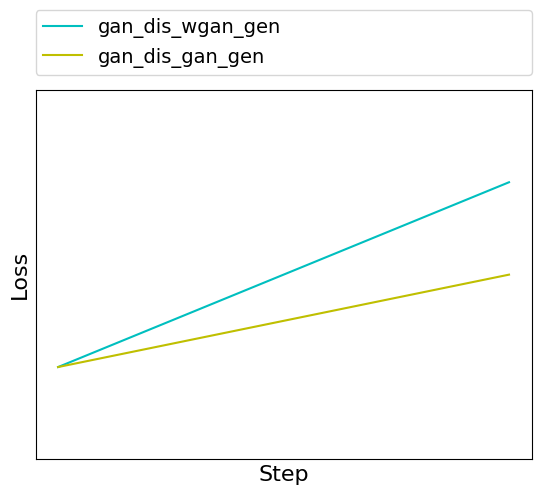
\includegraphics[width=0.5\textwidth]{figures/ex/wgan_wins_gan_dis}
		\caption{Both WGAN and GAN discriminators losses are bigger when competing against WGAN generator. A sign that the WGAN generator produces better images.}
		\label{fig:cd_wgan_wins}
	\end{figure}
	\begin{figure}[h!]
		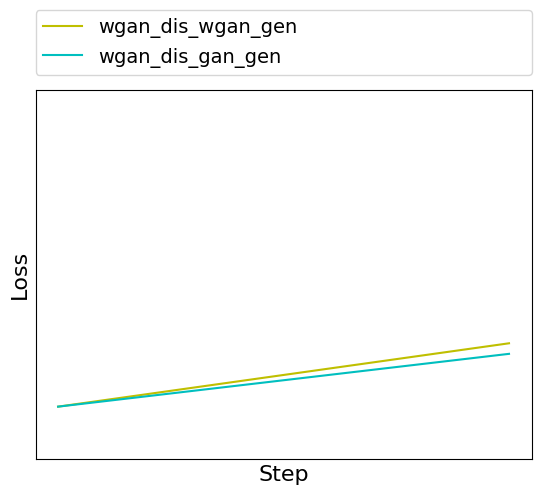
\includegraphics[width=0.5\textwidth]{figures/ex/equal_wgan_dis}
		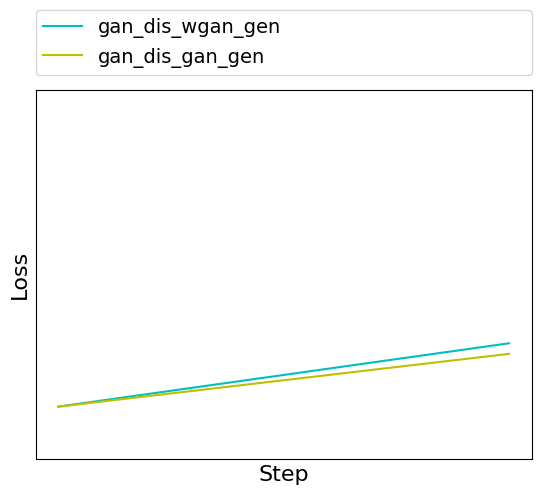
\includegraphics[width=0.5\textwidth]{figures/ex/equal_gan_dis}
		\caption{Both WGAN and GAN discriminators perform almost equally well on the both generators.}
		\label{fig:cd_equal}
	\end{figure}
	
	
However, it can also happen, that either a discriminator or a generator overfits in one or even both GANs. There are lots of possible combinations, here are some examples:
\begin{enumerate}
	\item Both generators overfit with respect to their own discriminators. This means, that they will be able to produce images that do not look better from a human perspective, but are tuned to fool the respective discriminator. In this case we will see graphs like in Figure~\ref{fig:cd_gen_overfit}.
	\item It is also possible that the discriminators overfit in a sense that instead of analyzing the structure of real images they remember peculiarities present in the images produced by their generators. In this scenario plots will resemble those shown in Figure~\ref{fig:cd_dis_overfit}.
	\item The trickiest case is when the WGAN discriminator overfits and at the same time the GAN generator, or vice versa. Unfortunately, as shown in Figure~\ref{fig:cd_gen_dis_overfit}, in this case the loss plots could look very similar to the case where WGAN generator just performs better.
\end{enumerate}

	\begin{figure}[h!] 
		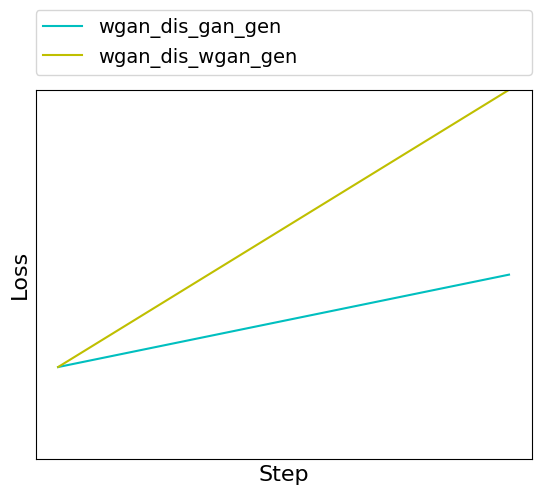
\includegraphics[width=0.5\textwidth]{figures/ex/gen_overfit_wgan_dis}
		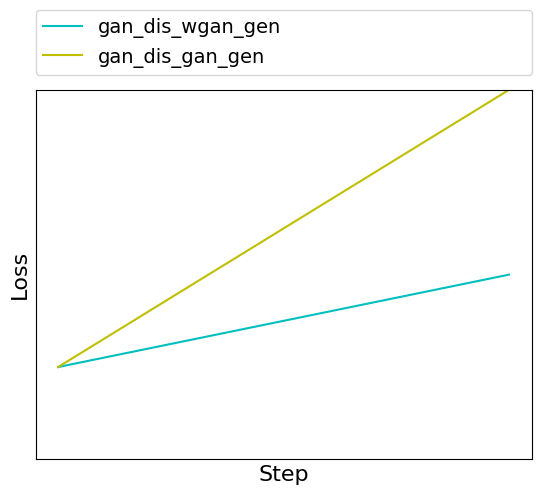
\includegraphics[width=0.5\textwidth]{figures/ex/gen_overfit_gan_dis}
		\caption{Both WGAN and GAN discriminators losses are bigger when competing against own generator. A sign that generators overfit against own discriminators.}
		\label{fig:cd_gen_overfit}
	\end{figure}
	\begin{figure}[h!] 
		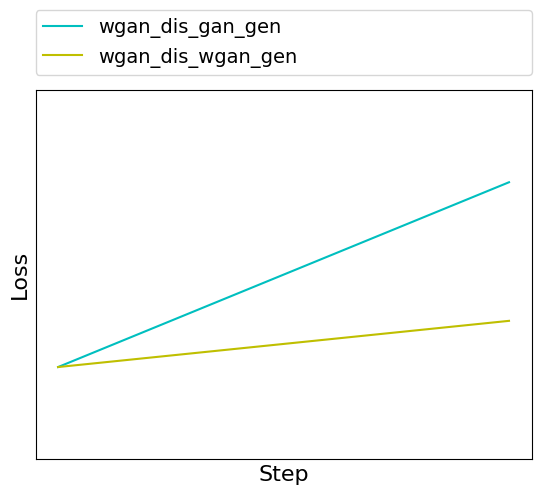
\includegraphics[width=0.5\textwidth]{figures/ex/dis_overfit_wgan_dis}
		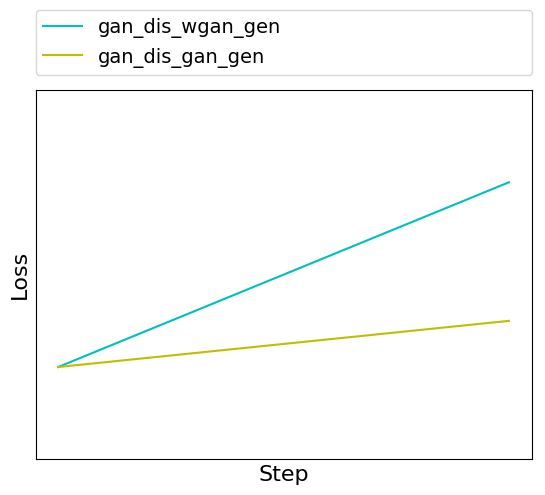
\includegraphics[width=0.5\textwidth]{figures/ex/dis_overfit_gan_dis}
		\caption{Both WGAN and GAN discriminators losses are bigger when competing against each other's generator. A sign that discriminators overfit against own generators.}
		\label{fig:cd_dis_overfit}	
	\end{figure}	
	\begin{figure}[h!] 
		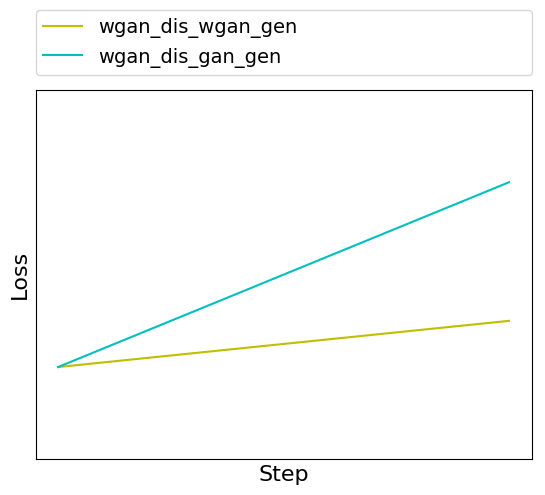
\includegraphics[width=0.5\textwidth]{figures/ex/gen_dis_overfit_wgan_dis}
		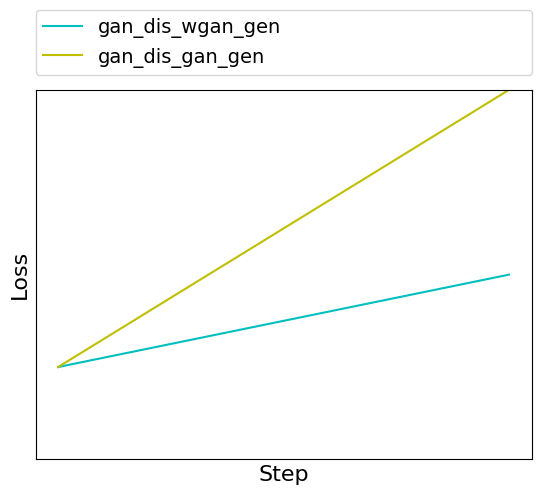
\includegraphics[width=0.5\textwidth]{figures/ex/gen_dis_overfit_gan_dis}
		\caption{Both the WGAN and GAN discriminators losses are bigger when competing against GAN generators. However, in this case the GAN discriminator and the WGAN generator overfit.}
		\label{fig:cd_gen_dis_overfit}
	\end{figure}
As we have seen, even in the case where one generator causes more problems for both discriminators, this can be a consequence of overfitting. So, normally, we would have to do additional tests to verify whether this is the case or not. Such a verification can be done by applying the same technique to two instances of the same network type, e.g. two WGANs. If after the additional verification we conclude that there is no overfitting, then we can finally claim that one generator performs relatively better. Moreover, in practice it turns out that multiple runs can produce different results even when using the same hyper-parameters. This happens because overfitting can be a result of a poor weight initialization. Therefore, each test has to be repeated several times and produce congruent results. 

There are several key differences when comparing this modified metric to the original generative adversarial metric. First, as already said, the GAM can not be applied to GANs whose discriminators do not output a valid probability distribution, which is the case with the WGAN. On the other hand, the GAM can be applied to a fully trained network, while each run of the modified metric requires both networks to be trained from scratch. However, as I have observed during my experiments, one has to train the networks several times due to occasional overfitting. Also, the modified metric provides information about the loss at different times of the training process. This can provide additional information, because if two networks change the lead multiple times during the training, it means that they can not be really compared.  

\subsection{Results}
The results of applying the modified generative adversarial metric are shown in Figure~\ref{fig:cd_wgan_vs_gan}. As we can see, after a significant amount of training steps the WGAN discriminator is able to distinguish images produced by its own and by the GAN discriminator equally well. On the other hand, the GAN discriminator almost constantly performs much better on its own generator. This may suggest that the GAN discriminator overfits. 
\begin{figure}[h!]
	\begin{subfigure}[b]{0.5\textwidth}
		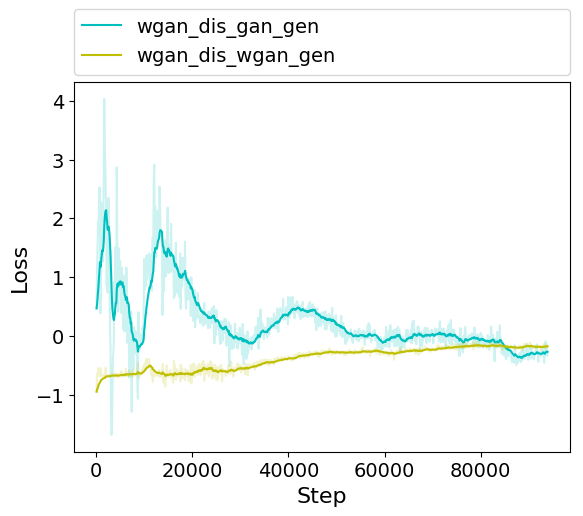
\includegraphics[width=\textwidth]{figures/cross_dis/trial16_wgan_dis_gan_gen}
	\end{subfigure}
	\begin{subfigure}[b]{0.5\textwidth}
		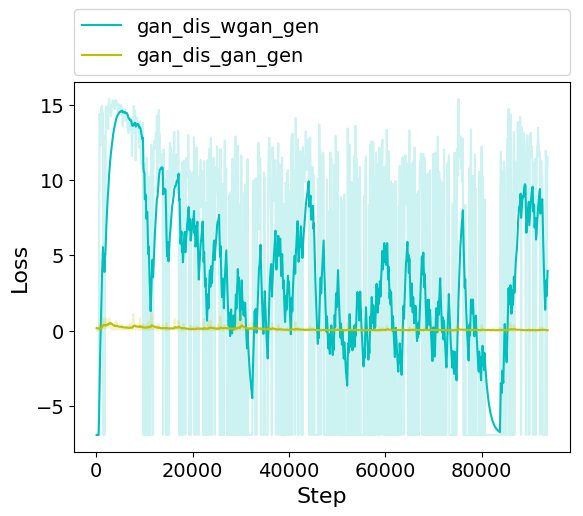
\includegraphics[width=\textwidth]{figures/cross_dis/trial16_gan_dis_wgan_gen}
	\end{subfigure}
	\caption{Results of applying the modified adversarial metric on a GAN and a WGAN. As we can see the GAN discriminator almost constantly performs worse when judging images produced by the WGAN generator, on the other hand the WGAN discriminator performs equally well on both generators.}
	\label{fig:cd_wgan_vs_gan}
\end{figure}

\begin{figure}[h!]
	\begin{subfigure}[b]{0.5\textwidth}
		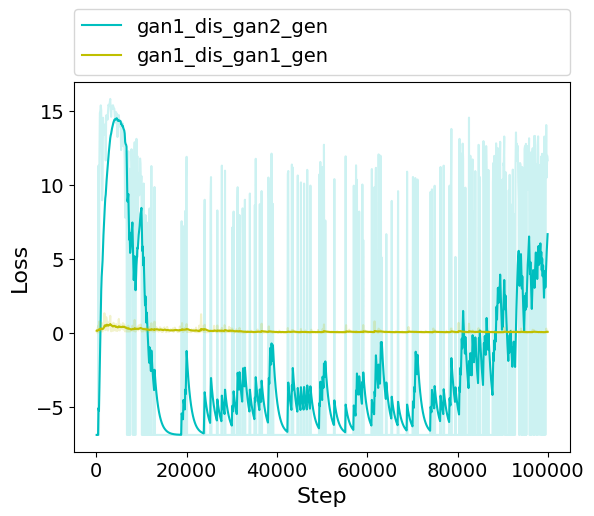
\includegraphics[width=\textwidth]{figures/cross_dis/trial15_gan1_dis_gan2_gen}
	\end{subfigure}
	\begin{subfigure}[b]{0.5\textwidth}
		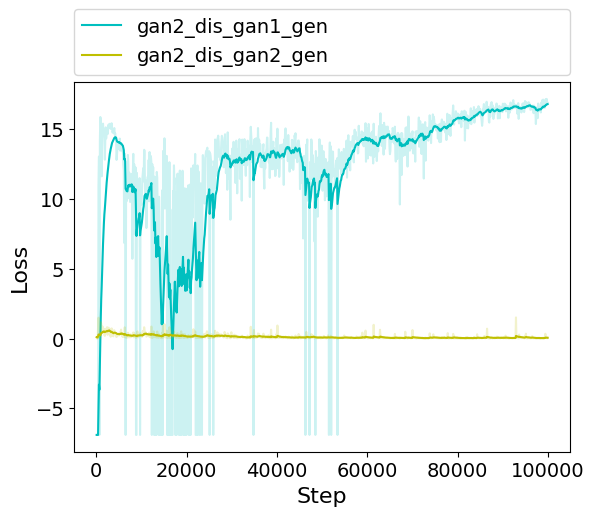
\includegraphics[width=\textwidth]{figures/cross_dis/trial15_gan2_dis_gan1_gen}
	\end{subfigure}
	\caption{Results of applying the modified adversarial metric on two GANs. Both discriminators can better distinguish images from their own generators}.
	\label{fig:cd_gan_vs_gan}
\end{figure}

To further investigate this hypothesis I have used the same metric to compare two GANs. The corresponding results are shown in Figure~\ref{fig:cd_gan_vs_gan}. While loss plots are oscillating, the trend is that after at some point of the training process GAN discriminator performs better on its own generator. On the other hand, when comparing two WGAN discriminators, it turned out that they perform equally well on both generators, as shown in Figure~\ref{fig:cd_wgan_vs_wgan}. All experiments were conducted several times and the corresponding plots can be found in Appendix~\ref{app:results}.
\begin{figure}[h!]
	\begin{subfigure}[b]{0.5\textwidth}
		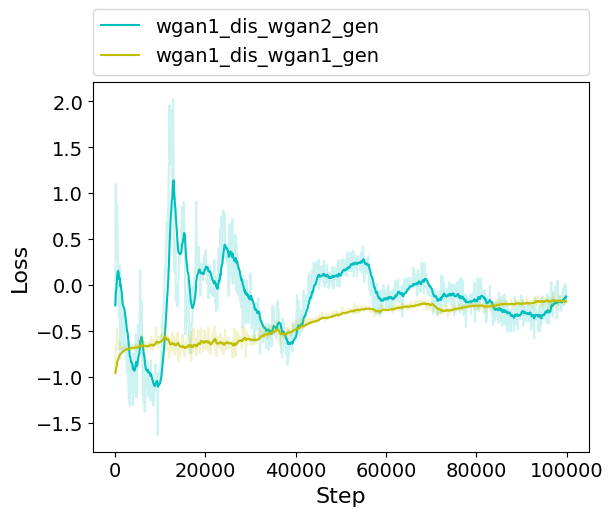
\includegraphics[width=\textwidth]{figures/cross_dis/trial17_wgan1_dis_wgan2_gen}
	\end{subfigure}
	\begin{subfigure}[b]{0.5\textwidth}
		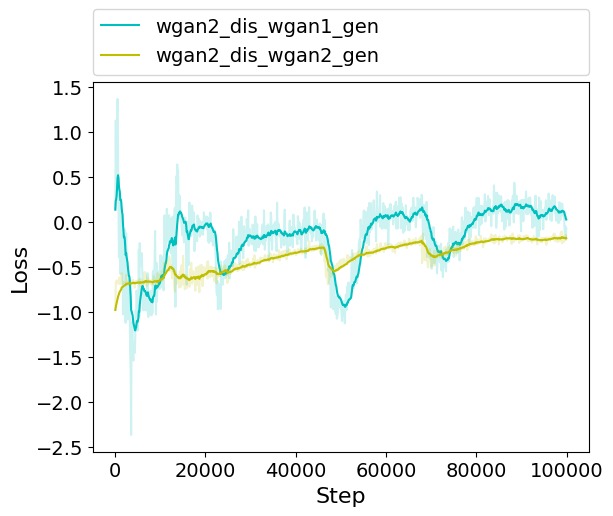
\includegraphics[width=\textwidth]{figures/cross_dis/trial17_wgan2_dis_wgan1_gen}
	\end{subfigure}
	\caption{Results of applying the modified adversarial metric on two WGANs. Both discriminators can better distinguish images from the foreign generator.}
	\label{fig:cd_wgan_vs_wgan}
\end{figure}

There are two main conclusions that can be drawn from the experiment results. Firstly, since the WGAN discriminator does not show any overfitting behavior, we can use its loss values when measuring both GAN and WGAN generators to claim that they both produce images of the same quality. Those who believe in their own ability to distinguish real and generates faces can take look at the samples generated by both generators, included in Appendix~\ref{app:results}. Furthermore, experiments suggest that the GAN discriminator overfits with respect to its own generator. Therefore, I have conducted more experiments to investigate the decision boundary learned by the GAN discriminator.

\begin{figure}[h]
	\centering
	
\includegraphics[scale=1]{figures/gan_found_image1}
	
\includegraphics[scale=1]{figures/gan_found_image2}
	
\includegraphics[scale=1]{figures/gan_found_image3}
	
\includegraphics[scale=1]{figures/gan_found_image4}
	\caption{Examples of images that the GAN discriminator considers real.}
	\label{fig:gan_found_images}
\end{figure}

\begin{figure}[h!]
	\includegraphics[width=\textwidth]{figures/diversity_gan2_real_dis_real_images}
	\caption{A visualization of how the GAN discriminator's confidence changes when we add a Gaussian noise to a real image sample.}
	\label{fig:changed_real_image_real_dis}
\end{figure}

\begin{figure}[h!]
	\includegraphics[width=\textwidth]{figures/diversity_gan2_fake_dis_gen_images}
	\caption{A visualization of how the GAN discriminator's confidence changes when we add a Gaussian noise to a generated image sample.}
	\label{fig:changed_gen_image_fake_dis}
\end{figure}

Once a discriminator is fully trained we can search for an image which discriminator will confidently mark as real. We can do it by using gradient descent over the image space, using the output of the discriminator as a loss function:
\begin{equation}
	I^* = \argmax_{I \in R^{64 \times 64 \times 64}} D(I).
\end{equation} 
However, using output directly will result in a very slow learning, because the output of discriminator on a newly initialized random image should be almost zero. Therefore, the sigmoid function used as an activation in the last layer will be saturated and the gradient will vanish. Instead, I used output before activation. Of coarse, the discriminator's output is not a convex function and has numerous local maxima. But by conducting the search multiple times with different initial images we have a chance to find a maxima that will give us a confidence near one. 

However, in practice it turned out that the GAN discriminator's confidence is equal to one almost on the whole image space and it constantly marked randomly generated images as real, like the ones shown in Figure~\ref{fig:gan_found_images}. To further investigate this phenomenon I have tried to add Gaussian noise with different variances to find out how much should I distort an image to decrease the discriminator's confidence:
\begin{align*}
	Z &\sim \mathcal{N}(0, \sigma^2) \\
	\hat{I} &= I + Z.
\end{align*} One would expect that the more noise is added to the image the less likely the discriminator will think the image is real. However, results demonstrated in Figures~\ref{fig:changed_real_image_real_dis} and~\ref{fig:changed_gen_image_fake_dis} suggest the opposite. When an image was distorted to an extent, where the underlying face was hardly visible, the GAN discriminator marked it as real with a confidence equal to one. These results suggest that the loss function of the GAN discriminator has many local minimas in the points corresponding to the generated faces and is equal to one in all the regions that were not observed during the training process. 

These results suggests that we should not use the discriminator network for classifying whether an image is real or not. This is because it does not learn the whole set of possible pictures but rather only those present in the training data set (positive examples) and those produced by its generator (negative examples). So, in the regions not observed during the training process its function can take some arbitrary values, in this case it was equal to one almost everywhere. The most important part of a GAN is the generator network and the discriminator exists only to help the generator to train. 

%\begin{figure}[h]
%	\begin{subfigure}[b]{0.5\textwidth}
%		\includegraphics[width=\textwidth]{figures/diversity_gan2_real_dis_gen_images_plot}
%	\end{subfigure}
%	\begin{subfigure}[b]{0.5\textwidth}
%		\centering
%		\includegraphics[width=0.45\textwidth]{figures/diversity_gan2_real_dis_gen_imgs_var0}
%		\includegraphics[width=0.45\textwidth]{figures/diversity_gan2_real_dis_gen_imgs_var30}
%		\includegraphics[width=0.45\textwidth]{figures/diversity_gan2_real_dis_gen_imgs_var50}
%		\includegraphics[width=0.45\textwidth]{figures/diversity_gan2_real_dis_gen_imgs_var90}
%	\end{subfigure}
%	\caption{Visualization of how GAN discriminator's confidence changes when we add Gaussian noise to a real image sample.}
%	\label{fig:changed_gen_image_real_dis}
%\end{figure}

%\begin{figure}[h]
%	\begin{subfigure}[b]{0.5\textwidth}
%		\centering
%		\includegraphics[scale=1]{figures/random_images_fake_1}
%		\includegraphics[scale=1]{figures/random_images_fake_2}
%		\caption{The images that the GAN discriminator considered fake.}
%	\end{subfigure}
%	\begin{subfigure}[b]{0.5\textwidth}
%		\centering
%		\includegraphics[scale=1]{figures/random_images_real_2}
%		\caption{The images that the GAN discriminator considered real.}
%	\end{subfigure}
%\end{figure}




	\section{Conclusion}
In this thesis we provided an implementation of a plan GAN and a Wasserstein GAN. Then we described  a method that can be used to compare these two networks. Although the proposed method requires some manual analysis we were able to come to a conclusion that the Wassersteing GAN does not improve the quality of produced image samples. However, as we showed, it has some advantages, like a loss function for the generator that corresponds to the quality of images produced by it. Also Wasserstein GANs less sensible to the choice of hyper-parameters than the plan GANs, which allows to reduce the time spent on finding the right setting. 

After applying the modified generative adversarial metric we could observe that the discriminator of a plan GAN overfits in a sense that it tries to remember who the images produced by its generator look like instead of trying to understand how the real faces should look like. We conducted more experiments to find an image that will be marked by the GAN discriminator as a real one by searching on the whole image space. It turned out that the GAN discriminator considers a random noise image as a real one, which suggests that its computed function is equal to one almost on the whole domain. Also, in another experiment we came to a conclusion that after adding a sufficient amount of noise to a generated image the discriminator start to mark it as a real one. All these results mean that the discriminator should be used only to train the generator network and is useless on its own.
 
During the writing of this paper a new, improved version of a Wasserstein GAN was published~\cite{improved_wgan}. In their work the authors tried another method to enforce the Lipschitz constraint of the discriminator. Instead of weight clipping they penalized the norm of the discriminator gradients. Moreover, a new GAN architecture was published in April 2017, which uses a variational auto-encoder as a discriminator~\citep{alexnet}. The authors were able to double the resolution of the generated images and used the Inception metric to show that their model performs better on the CIFAR-10 data set. It would be interesting to apply the metric proposed in this paper to try to analyze these two new GANs. 
\end{spacing}
\newpage
\thispagestyle{empty}
\null

\newpage
\addcontentsline{toc}{section}{List of figures}
\listoffigures

%\input{appendices}

	
% Generierung des Literaturverzeichnisses
\bibliographystyle{IEEEtran}
\bibliography{references}

\newpage
\appendix 

\section{Experiment results} \label{app:results}

\begin{figure}[h!] 
	\begin{subfigure}[b]{\textwidth}		
		\includegraphics[width=0.5\textwidth]{figures/cross_dis/trial19_wgan_dis_gan_gen}
		\includegraphics[width=0.5\textwidth]{figures/cross_dis/trial19_gan_dis_wgan_gen}
	\end{subfigure}
	\begin{subfigure}[b]{\textwidth}		
		\includegraphics[width=0.5\textwidth]{figures/cross_dis/trial18_wgan_dis_gan_gen}
		\includegraphics[width=0.5\textwidth]{figures/cross_dis/trial18_gan_dis_wgan_gen}
	\end{subfigure}
	\begin{subfigure}[b]{\textwidth}		
		\includegraphics[width=0.5\textwidth]{figures/cross_dis/trial16_wgan_dis_gan_gen}
		\includegraphics[width=0.5\textwidth]{figures/cross_dis/trial16_gan_dis_wgan_gen}
	\end{subfigure}
		\caption{A WGAN vs a GAN. The GAN discriminator's loss values are plotted using the logarithmic scale.}
\end{figure}

\begin{figure}[h!] 
	\begin{subfigure}[b]{\textwidth}		
		\includegraphics[width=0.5\textwidth]{figures/cross_dis/trial15_gan1_dis_gan2_gen}
		\includegraphics[width=0.5\textwidth]{figures/cross_dis/trial15_gan2_dis_gan1_gen}
	\end{subfigure}
	\begin{subfigure}[b]{\textwidth}		
		\includegraphics[width=0.5\textwidth]{figures/cross_dis/trial14_gan1_dis_gan2_gen}
		\includegraphics[width=0.5\textwidth]{figures/cross_dis/trial14_gan2_dis_gan1_gen}
	\end{subfigure}
	\caption{A GAN vs another GAN. Loss values are plotted using the logarithmic scale.}
\end{figure}

\begin{figure}[h!] 
	\begin{subfigure}[b]{\textwidth}		
		\includegraphics[width=0.5\textwidth]{figures/cross_dis/trial17_wgan1_dis_wgan2_gen}
		\includegraphics[width=0.5\textwidth]{figures/cross_dis/trial17_wgan2_dis_wgan1_gen}
	\end{subfigure}
	\caption{A WGAN vs another WGAN.}
\end{figure}

\begin{figure}[h]
	\includegraphics[scale=1.0]{figures/wgan_palette}
	\caption{Sample images produced by a WGAN generator}
\end{figure}


\begin{figure}[h]
	\includegraphics[scale=1.0]{figures/gan_palette}
	\caption{Sample images produced by a GAN generator}
\end{figure}

\end{document}
